\documentclass[titlepage, 11pt]{scrartcl}
\usepackage{graphicx}
\usepackage[utf8]{inputenc}
\usepackage{hyperref}
\usepackage{amsmath, amsthm, amsfonts}
\usepackage{graphics}
\usepackage{skull}
\usepackage{mathabx}
\usepackage{float}
\usepackage{epsfig}
\usepackage{amssymb}
\usepackage{dsfont}
\usepackage{latexsym}
\usepackage{newlfont}
\usepackage{epstopdf}
\usepackage{amsthm}
\usepackage{epsfig}
\usepackage{caption}
\usepackage{multirow}
\usepackage{graphics}
\usepackage{wrapfig}
\usepackage[rflt]{floatflt}
\usepackage{multicol}
\usepackage{minted}

\hypersetup{colorlinks,%
	citecolor=black,%
	filecolor=cyan,%
	linkcolor=blue!60,%
	urlcolor=cyan}

\title{
    \normalfont\normalsize
    {\huge Modelos de Optimización\\
    		\textbf{Laboratorio 8:}  Búsqueda Bibliográfica de Metaheurísticas eficientes para 
    		la solución de problemas de optimización en enteros
}
    \vspace{12pt}
}

\author{Osmany P\'erez Rodr\'iguez\\
		Enrique Mart\'inez Gonz\'alez\\
		Carmen Irene Cabrera Rodr\'iguez\\
		\textbf{Grupo C412}}
	

\date{}

\begin{document}
    \maketitle 
    
    \section{Metaheurísticas}
		El término \textit{heurística} se refiere a una técnica basada en la experiencia y el sentido común para determinar una buena aproximación al óptimo de un problema de forma eficiente.
		
		Una metaheurística sería un método heurístico no dependiente de un problema particular, sino diseñado para resolver un tipo de problema computacional general, usando los parámetros que brinda el usuario sobre unos procedimientos genéricos y abstractos. La mayoría de ellas están conformadas por reglas que simulan un fenómeno o proceso de la Física o la Biología, y por tanto, se interpretan conforme a dicho proceso.Usualmente, estas se aplican a problemas que no tienen un algoritmo o heurísitca específica que produzca una solución satisfactoria; o bien cuando no es posible implementar ese método óptimo. Resultan de gran utilidad en problemas de optimización difíciles por su complejidad computacional o de muy grandes dimensiones.
		
		Es posible combinar diferentes metaheurísticas con el fin de compensar las debilidades de algunas con las ventajas de otras. A continuación se ofrece un resumen de algunas metaheurísticas utilizadas.

	    \subsection{Recocido Simulado}
	    	El nombre de este algoritmo viene del proceso de recocido del acero y cerámicas, una técnica que consiste en calentar y luego enfriar lentamente el material para variar sus propiedades físicas y alcanzar su estado de mínima energía.
	    	
	    	Se asume que se tiene un sistema de vecindades dado por la aplicación tal que para cada elemento $x$ del espacio de búsqueda se le asocia un subconjunto $V(x)$ del mismo. 
	    	En cada iteración, se tiene un estado $s$ que está conformado por una solución actual $x_k$, siendo $k$ el número de la iteración, más los parámetros de entrada, con sus respectivos valores dada la iteración. El método evalúa algunos vecinos del estado actual $s$ y probabilísticamente decide entre efectuar una transición a un nuevo estado $s'$ o quedarse en el estado $s$.La comparación entre estados vecinos se repite hasta que se encuentre un estado óptimo que minimice la energía del sistema o hasta que se cumpla cierto criterio de parada.
	    	
	    	\subsubsection{Pseudocódigo}
	    		Parámetros iniciales:
	    		\begin{itemize}
	    			\item Temperatura inicial ($t_0$)
	    			\item Período o número de soluciones evaluadas para una temperatura dada ($L$).
	    			\item Estrategia de enfriamiento o disminución de la temperatura.
	    			\item Temperatura final ($t_f$)
	    		\end{itemize}
    			
    			Además es necesario:
    			\begin{itemize}
    				\item Definir el sistema de vecindades $V(x), \ \forall x \in S$
    				\item Seleccionar un punto inicial $x_0$
    			\end{itemize}
    		
    		El algoritmo funciona como sigue:
    		\begin{figure}[H]
    			\begin{minted}[tabsize=4]{python}
def SimulatedAnnealing(t0, x0, L, t_final):
	# Best solution found at the moment
	x_best = x0 
	
	t = t0
	x = x0
	while t <= t_final:
		k = 0
		while k <= L:
			y = GenerateElementIn(V, x)
			
			delta = f(y) - f(x)
			if delta <= 0:
				x = y
				if f(y) < f(x_best):
					x_best = y
			
			else: # delta > 0
				r = random(0, 1)
				if r <= exp(- delta / t):
					x = y
			
			k = k + 1
		
		t = Decrease(t)
		
	return x_best
			\end{minted}
			\caption{Pseudocódigo para el algoritmo de Recocido Simulado}.
		\end{figure}
	
		\subsubsection{Observaciones}
			Note que aunque el valor de la función no mejora para el nuevo candidato $y$; el algoritmo aún puede aceptarlo de acuerdo a una cierta probabilidad (Ley de distribución de Boltzmann), que depende de la temperatura actual del proceso. Una temperatura más alta hace que sea más probable aceptarlo o no.
			
			Este es el factor clave del método, puesto que es el que permite salir de un mínimo local y de ese modo, diversificar la exploración, para finalmente poder alcanzar el mínimo global. Usualmente se toma la temperatura inicial bastante alta, para que al inicio se puedan aceptar más candidatos, incluso los que empeoran la evaluación de la función.
			
			En cuanto a los criterios de parada, bajo la estrategia descrita anteriormente, hay dos que son los más utilizados:
			\begin{itemize}
				\item Fijar un número máximo de iteraciones a realizar
				\item Si la variación en el valor de la función objetivo no es significativo en cierto número de iteraciones se decide parar.
			\end{itemize}
	    

	    \subsection{Búsqueda Tabú}
			Este es un método de búsqueda local determinista que prohíbe ciertos movimientos que se denominan \textit{movimientos prohibidos o tabú}. Este hace uso de estructuras de memoria, no solo para conservar la mejor solución, sino la información sobre el itinerario que conduce a ella; de esta forma, una vez que una potencial solución es determinada se la marca como tabú para que el algoritmo no vuelva a visitarla.
			
			Entre dichas estructuras se halla la \textit{lista tabú} integrada por los movimientos prohibidos y que se actualiza durante la ejecución del código. Esta lista tiene carácter dinámico puesto que un movimiento permanece prohibido solo por un cierto número de iteraciones, luego se permite.
			
			\subsubsection{Pseudocódigo}
			Los parámetros de entrada serían:
			\begin{itemize}
				\item Punto inicial $x_0$
				\item Tamaño de la lista tabú $n$. Este valor también es llamado tenor del tabú.
			\end{itemize}
			
			El algoritmo funciona como sigue:
			\begin{figure}[H]
				\begin{minted}[tabsize=4]{python}
def TabuSearch(x0, n):
	# Best solution found 
	x_best = x0
	
	x = x0
	tabuList = [x0]
	
	while not stoppingCondition():
		x_neighbors = getNeighbors(x)
		x_best_candidate = x_neighbors[0]
		for x_candidate in x_neighbors:
			if (x_candidate not in tabuList
				and fitness(x_candidate) > fitness(x_best_candidate)):
				x_best_candidate = x_candidate
		x = x_best_candidate
		
		if fitness(x) > fitness(x_best):
			x_best = x
		
		tabuList.append(x)
		if len(tabuList) > n:
			tabuList.RemoveFirst()
	
	return x_best

				\end{minted}
				\caption{Pseudocódigo para el algoritmo de Búsqueda Tabú}.
			\end{figure}
		    
		    Los criterios de parada pueden ser:
		    \begin{itemize}
		    	\item Número máximo de iteraciones.
		    	\item La función objetivo no ha cambiado significativamente su valor luego de cierto número de iteraciones.
		    	\item El valor de la función objetivo es aceptable.
		    \end{itemize}
	    
	    	\subsubsection{Observaciones}
	    		La función \textit{fitness} (función de aptitud) es generalmente una función matemática que devuelve una puntuación o si se cumplen los criterios de aspiración; por ejemplo un criterio de aspiración podría ser encontrar un nuevo espacio de búsqueda. Si el mejor candidato local tiene un valor de aptitud más alto que el mejor actual, este se establece como el nuevo mejor.
			    Note, que el procedimiento seleccionará al mejor candidato local ($x\_best\_candidate$), aunque tenga peor aptitud que el $x\_best$ para escapar del óptimo local.
	    
	    \subsection{Algoritmos genéticos (AG)}
	    	Estos algoritmos reciben su nombre por estar inspirados en la evolución biológica y su base genético-molecular. Se hace evolucionar una población de individuos, sometiéndola a acciones aleatorias como mutaciones o recombinaciones genéticas; así como a una selección de acuerdo a algún criterio, que decide cuáles son los que sobreviven y cuáles los descartados.
	    	
	    	Se considera un subconjunto del espacio de búsqueda, donde cada elemento representa un cromosoma (cada cromosoma define a un individuo). Para realizar la exploración se definen los siguientes operadores, bajo criterios probabilísticos:
	    	\begin{description}
	    		\item[Operador de cruzamiento (Cross)] Dados dos cromosomas \textit{padres} se obtiene uno nuevo con características de sus padres o igual a uno de ellos.
	    		\item[Operador de mutación (Mutate)] Dado un cromosoma, se realiza un cambio en él para generar uno nuevo.
	    		\item[Operador de selección (Select)]: Decide si un individuo pasa o no a la siguiente generación.
	    	\end{description}
	    	
	    	\subsubsection{Pseudocódigo}
	    		Se pasa como parámetro de entrada:
	    		\begin{itemize}
	    			\item Tamaño de la población inicial $n$
	    		\end{itemize}
    		
    			Igualmente es necesario definir la probabilidad de mutación, la probabilidad de cruzamiento y el número de generaciones a estudiar en el proceso evolutivo, así como los criterios para la selección de la nueva generación; de modo que se puedan formular los operadores antes mencionados.
	    		
    			El algoritmo funciona como sigue:
	    		\begin{figure}[H]
	    			\begin{minted}[tabsize=4]{python}
def GeneticAlgorithm(n):
	P = GenerateInitialPopulation(n)

	# Best solution found 
	x_best = MinCost(P)
	
	while not stoppingCondition():
		count_mutate = CalculateMutations()
		count_crossing = CalculateCrossings()
		
		P_to_mutate = SelectToMutate(P, count_mutate)
		new_chroms = Mutate(P_to_mutate)
		
		P_to_cross = SelectToCross(P, count_crossing)
		pairs = GeneratePairs(P_to_cross)
		
		new_chroms += Cross(pairs)
		
		P = Select(new_chroms)
		x_best = min(x_best, MinCost(P))
		    	
	    			\end{minted}
	    			\caption{Pseudocódigo para el Algoritmo Genético}.
    			\end{figure}
	    	
	    		Se pueden establecer como criterios de parada los siguientes:
	    		\begin{itemize}
	    			\item Establecer un número máximo de generaciones
	    			\item Obtener un cromosoma cuyo costo es inferior a cierto valor de umbral prefijado
	    			\item No obtener una disminución significativa de la función de costo durante cierto número de generaciones.
	    		\end{itemize}
    		
    		\subsubsection{Observaciones}
    			Si cuando se realiza la selección de los cromosomas, se eligen siempre los de menor costo, esto puede provocar que las poblaciones se parezcan mucho entre sí y estancar el procedimiento en soluciones aparentemente buenas (efecto hemofílico).
    			
    			Igualmente, al seleccionar la población inicial, si esto no se hace de forma aleatoria, es importante garantizar que dentro de ella se tenga diversidad estructural, para tener una representación de la mayor parte de la población posible.
	    
	    
	    
	    \subsection{Inteligencia de enjambres. Algoritmo de la colonia de hormigas}
	    	La inteligencia de enjambres es una rama de la inteligencia artificial que estudia el comportamiento colectivo de los sistemas descentralizados, autoorganizados, naturales o artificiales. Están inspirados por ciertos sistemas biológicos de la naturaleza conformados por una población de agentes simples que interactúan entre ellos y con el medio ambiente. Tal es el caso de: las colonias de hormigas, el alineamiento de las aves en vuelo, el comportamiento de rebaños durante el pastoreo y el crecimiento bacteriano.
	    	
	    	El algoritmo de la colonia de hormigas (ACO - \textit{Ant Colony Optimization}) es una técnica probabilística para solucionar problemas computacionales que pueden reducirse a buscar los mejores caminos o rutas en grafos.
	    	
			La idea del mismo proviene de la observación de la explotación de los recursos alimentarios entre hormigas, las cuales son capaces, en conjunto de buscar el menor camino existente entre la fuente de comida y su colonia.
			
			La primera hormiga encuentra la fuente de alimentos ($F$) a través de cualquier camino ($a$), y retorna a la colonia ($N$) dejando un rastro de feromonas tras de sí. Las hormigas más cercanas se verán atraídas por ellas y seguirán su pista de forma más o menos directa. De este modo, al regresar a la colonia habrán fortalecido de feromonas la ruta más corta, haciéndola más atractiva, y dado que las feromonas son volátiles, aquellas que estaban en la ruta más larga irán desapareciendo. Finalmente todas habrán escogido el camino más corto.
			
			\subsubsection{Pseudocódigo}
				\begin{figure}[H]
					\begin{minted}[tabsize=4]{python}
def ACO():
	Initialize()
	while not StoppingCriterion():
		P = PositionAnts(starting_node)
		while True:
			for ant in P:
				ChooseNextNode(ant)
				UpdatePheromone(ant)
			if AllAntsReachSolution(P):
				break
		UpdateBestSolution()
		ApplyPheromoneUpdate()		
	    			\end{minted}
	    			\caption{Pseudocódigo para el algoritmo de la colonia de hormigas}.
    			\end{figure}
    		
    		\subsubsection{Observaciones}
    			Para la selección de aristas en el camino, cada hormiga computa un conjunto de expansiones factibles de su estado actual y se mueve a una de ellas de forma probabilística, que depende del \textit{atractivo} del movimiento, computado por alguna heurística que indica a priori la conveniencia de dicho movimiento, y el \textit{nivel de rastro} del movimiento. Los rastros son actualizados cuando todas las hormigas han actualizado su solución, que depende de la cantidad de feromonas depositadas por las hormigas.
		    
 	\section{Problema del viajante}
 	
 		Sobre una red de carreteras que conecta $n$ ciudades $C_1, \ldots, C_n$ se desea el itinerario de mínima distancia que partiendo de una ciudad, pasa una sola vez por todas y cada una de las ciudades, volviendo a la ciudad inicial.
 		
 		\subsection{Modelo}
 			\textbf{Parámetros:} $d_{ij} \rightarrow$ distancia netre la ciudad $i$ y la ciudad $j$.
 			
 			\textbf{Variables:}
 			$ C_{ijk} = 
 			\begin{cases}
 				1 & \text{si en el momento $k$ se va de la ciudad $i$ a la $j$}\\
 				0 & \text{si no}
 			\end{cases}$
 			
 			\textbf{Modelo:}
 			\begin{align*}
 				min \sum_{i, j, k = 1}^{n} C_{i, j, k}d_{ij}\\
 				s.a \sum_{i = 1}^{n}C_{1, i, 1} &= 1\\
 				\sum_{i, j = 1}^{n}C_{i, j, k} &= 1, \ k = 2, \ldots, n\\
 				\sum_{j, k = 1}^{n}C_{i, j, k} &= 1, \ i =  1, \ldots, n\\
 				\sum_{i = 1}^{n} C_{i, j, k} - \sum_{i = 1}^{n}C_{i, j, k+ 1} = 0, \ j &= 1, \ldots, n; \ k = 1, \ldots, n - 1\\
 				\sum_{i = 1}^{n} C_{i, 1, n} &= 1
 			\end{align*}
 	
 		\subsection{Algoritmo utilizado}
 			Para resolver este problema se utilizó la biblioteca de Python \href{https://acopy.readthedocs.io/en/latest/readme.html}{ACOpy} que implementa el algortimo de la colonia de hormigas (ACO - Ant Colony Optimization). Permite, entre otros \textit{features}, personalizar el solucionador de acuerdo a ciertos parámetros y tracear información sobre el proceso de resolución.
 			
 			\subsubsection{Código empleado}
 				\begin{figure}[H]
	 				\begin{minted}[tabsize=4]{python}
def ant_colony_optimization_tsp(matrix,rho=.03,q=1,alpha=1,beta=3):
	G = nx.Graph(matrix)
	solver = acopy.Solver(rho=rho, q=q)
	colony = acopy.Colony(alpha=alpha, beta=beta)
	
	solver.add_plugin(acopy.plugins.Printout())
	solver.add_plugin(acopy.plugins.Timer())
	solver.add_plugin(acopy.plugins.StatsRecorder())
	
	path = solver.solve(G, colony, limit=100)
	
	t = solver.plugins['Timer']
	print('Time per iter:')
	print(t.time_per_iter)
	print('Duration:')
	print(t.duration)
	
	return (path, solver, colony)
	 				\end{minted}
	 				\caption{Puede acceder al código completo a través de este \href{viajante.py}{enlace}}.
 				\end{figure}
 			
 				Note que se genera una colonia de hormigas con los parámetros:
 				\begin{description}
 					\item[alpha(float)] Factor relativo para la feromona en las aristas; representa cuánto importa la feromona para la hormiga.
 					\item[beta(float)] Factor relativo para el costo de las aristas; representa cuánto importa la distancia.
 				\end{description}
 				Las hormigas exploran el grafo utilizando $alpha$ y $beta$ en el proceso de decisión para determinar cuál será la siguiente arista a la que se moverán.
 				
 				De igual forma, se setea el solucionador con los parámetros:
 				\begin{description}
 					\item[q(float)] Cantidad de feromona a depositar en las aristas.
 					\item[rho(float)] El porciento de feromona a evaporar.
 				\end{description}
 		
 		\subsection{Resultados obtenidos}
 		Tomando una cantidad $n = 10$ de ciudades, se obtuvieron los siguientes resultados:
		\begin{figure}[H]
			\begin{minted}[tabsize=4]{bash}

Using 10 ants from Colony(alpha=1, beta=3)
Performing 100 iterations:
Iteration  Cost                 Solution
1          385                  0 1 9 8 7 6 5 4 3 2
2          342                  0 3 8 6 5 4 2 7 9 1
3          308                  0 3 8 9 6 2 7 5 4 1
4          279                  0 1 4 2 7 5 9 6 8 3
5          258                  0 3 8 5 4 2 7 6 9 1
7          255                  0 1 4 2 7 9 6 5 3 8
12         243                  0 3 8 5 9 6 7 2 4 1
13         234                  0 3 8 2 7 6 9 5 4 1
16         227                  0 1 4 5 3 8 9 6 7 2
25         211                  0 1 4 2 7 6 9 5 3 8
36         202                  0 1 4 5 3 8 2 7 6 9
---------------------------------------------------
Time per iter:
0.004998197555541992
Duration:
0.4998197555541992

			\end{minted}
		\end{figure}
		Vea que la última fila de la tabla anterior muestra el valor que alcanza la función en la columna \textbf{Cost} y el vector solución (la permutación para la que se obtiene dicho costo) en la columna \textbf{Solution}
 		
 		\subsection{Comparación de la metaheurística utilizada con las metodologías de planos cortantes y ramificación y acotación}
 			La mayoría de los problemas combinatorios de optimización resultan difíciles de resolver. Los algoritmos exactos, como las metodologías de planos cortantes y ramificación y acotación, garantizan que se hallará una solución óptima al problema; sin embargo, el tiempo de ejecución de estos algoritmos crece de forma dramática cuando aumenta el tamaño de la instancia del problema.
 			
 			Desde un punto de vista teórico, es posible resolver cualquier problema lineal en enteros usando un acercamiento con los métodos de planos cortantes. No obstante, puede demorar un largo tiempo la convergencia al óptimo; en parte, porque el subproblema de separar cortes efectivos ya resulta complicado. Es por ello, que en numerosas ocasiones se recurre a la combinación de este con otros métodos, como es el caso del de ramificación y acotación: Se generan cortes en los nodos del árbol de ramificación y acotación, para estrechar los límites de las relajaciones LP o para excluir soluciones no factibles. De hecho, en los ejemplos que se mostrarán a continuación, el solucionador utilizado es CBC (\textit{COIN-OR Branch-and-Cut}) de la biblioteca MIP de Python, que es la combinación de dichos algoritmos.
 			
 			Cuando se está en presencia de los casos en que los algoritmos exactos no son los más efectivos, es que se recurre a las diferentes heurísticas, que intercambian la optimalidad de la solución por un mejor tiempo de ejecución; es decir, están diseñadas para obtener soluciones buenas pero no necesariamente óptimas en un tiempo aceptable. 
 			
 			En particular, en el caso del algoritmo de la colonia de hormigas, la retroalimentación positiva conduce a un rápido descubrimiento de buenas soluciones. A diferencia de otras metaheurísitcas, como los algoritmos genéticos, la computación distribuida evita la convergencia prematura. Aunque es cierto que se garantiza la convergencia del método, el tiempo que demora en converger es incierto; por lo que se recurre a criterios de parada que pueden provocar que la solución obtenida no sea la óptima, tal como se mencionaba anteriormente.
 			
 			Utilizando las dos variantes de solución propuestas, se computó la solución del problema del viajante con varios valores de $n$(en orden ascendente); lo que permitió evaluar el tiempo de ejecución de los algoritmos y la optimalidad de las soluciones obtenidas. Los resultados fueron los siguientes:
 			
 			\begin{figure}[H]
				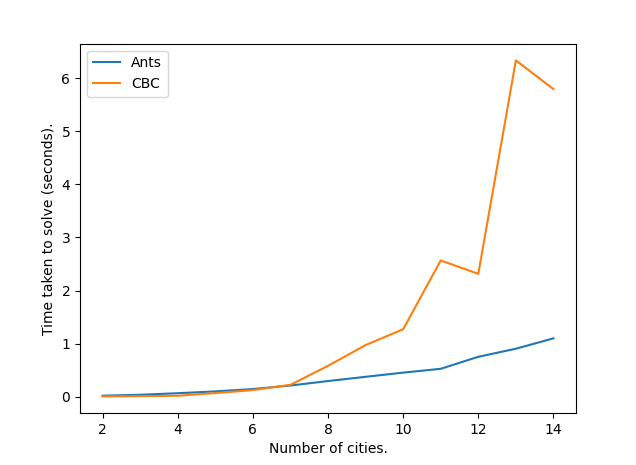
\includegraphics[]{pictures/ExecutionTime.png}
				\caption{Comparación del tiempo de ejecución.}
 			\end{figure}
 			\begin{figure}[H]
 				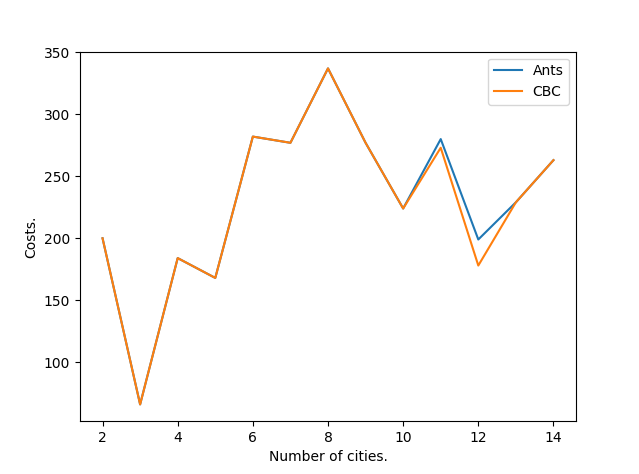
\includegraphics[]{pictures/Optimality.png}
 				\caption{Comparación de la optimalidad.}
 			\end{figure}
 			
			Puede acceder al código que genera estas gráficas a través del siguiente \href{main.py}{enlace}
			
			Como era de esperar, se puede observar que a medida que aumenta la cantidad de ciudades ($n$), los valores que retorna el algoritmo de la colonia de hormigas no son los óptimos, pero tampoco se encuentran muy alejados de la solución que devuelve el otro; además, el tiempo que demora el cómputo es mucho mejor que el del CBC.

 		

\end{document}